\documentclass{article}

% if you need to pass options to natbib, use, e.g.:
%     \PassOptionsToPackage{numbers, compress}{natbib}
% before loading neurips_2019

% ready for submission
% \usepackage{neurips_2019}

% to compile a preprint version, e.g., for submission to arXiv, add add the
% [preprint] option:
    % \usepackage[preprint]{neurips_2019}

% to compile a camera-ready version, add the [final] option, e.g.:
\usepackage[final]{neurips}

% to avoid loading the natbib package, add option nonatbib:
    % \usepackage[nonatbib]{neurips_2019}
\usepackage{multicol}
\usepackage{float}
\usepackage[center]{caption}

\usepackage[utf8]{inputenc} % allow utf-8 input
\usepackage[T1]{fontenc}    % use 8-bit T1 fonts
\usepackage{hyperref}       % hyperlinks
\usepackage{url}            % simple URL typesetting
\usepackage{booktabs}       % professional-quality tables
\usepackage{amsfonts}       % blackboard math symbols
\usepackage{nicefrac}       % compact symbols for 1/2, etc.
\usepackage{microtype}      % microtypography
\usepackage{graphicx}
\usepackage{amsmath}
\usepackage{xepersian}

\settextfont{XB Yas.ttf}

\title{تمرین شماره ۱ - قضیه CAP}


% The \author macro works with any number of authors. There are two commands
% used to separate the names and addresses of multiple authors: \And and \AND.
%
% Using \And between authors leaves it to LaTeX to determine where to break the
% lines. Using \AND forces a line break at that point. So, if LaTeX puts 3 of 4
% authors names on the first line, and the last on the second line, try using
% \AND instead of \And before the third author name.

\author{%
  امیرحسین مهدی‌نژاد\\
  شماره دانشجویی 810800058\\
  \texttt{mahdinejad@ut.ac.ir} \\
  % examples of more authors
  % \And
  % Coauthor \\
  % Affiliation \\
  % \texttt{email} \\
  % \AND
  % Coauthor \\
  % Affiliation \\
  % Address \\
  % \texttt{email} \\
}

% create title (includes both anonymized and non-anonymized versions)
% \providecommand{\@makepertitle}{}
% \newcommand{\makepertitle}{%
%   \vbox{%
%     \hsize\textwidth
%     \linewidth\hsize
%     \vskip 0.1in
%     \toptitlebar
%     \centering
%     {\LARGE\bf \@title\par}
%     \bottomtitlebar
%       \def\And{%
%         \end{tabular}\hfil\linebreak[0]\hfil%
%         \begin{tabular}[t]{c}\bf\rule{\z@}{24\p@}\ignorespaces%
%       }
%       \def\AND{%
%         \end{tabular}\hfil\linebreak[4]\hfil%
%         \begin{tabular}[t]{c}\bf\rule{\z@}{24\p@}\ignorespaces%
%       }
%       \begin{tabular}[t]{c}\bf\rule{\z@}{24\p@}\@author\end{tabular}%
%     \vskip 0.3in \@minus 0.1in
%   }
% }

\begin{document}


\begin{minipage}{0.1\textwidth}% adapt widths of minipages to your needs

\includegraphics[width=1.1cm]{Photos/UT_logo.png}
\end{minipage}%
\hfill%
\begin{minipage}{0.9\textwidth}\raggedleft
دانشکده فنی، دانشگاه تهران\\
سیستم‌های توزیع شده - 
آذر
ماه 1400\\
\end{minipage}
% \end{}


\makepertitle


% \begin{abstract}
%  این بخش از یک پاراگراف تشکیل شده است که توضیحاتی کلی در مورد مساله و راه حل شما ارائه می‌دهد.
% \end{abstract}
\begin{multicols}{2}
\section{قضیه \lr{CAP}}
یکی از مزایای استفاده از سیستم‌های توزیع‌شده، قابلیت اتکای بیشتر آن‌ها نسبت به سیستم‌های یکپارچه است.
ولی برای این قابلیت اتکا یا اطمینان، حدودی وجود دارد که در تئوری 
\lr{CAP}
با توجه به فاکتورهای زیر به صورت رسمی بیان می‌شود:
\begin{itemize}
    \item سازگاری
    \lr{(Consistency)} \\
    اگر همه‌ی نودهای یک سیستم، داده‌های یکسان را در یک زمان ببینند، آن سیستم سازگار خوانده می‌شود. 
    \begin{figure}[H]
        \center
        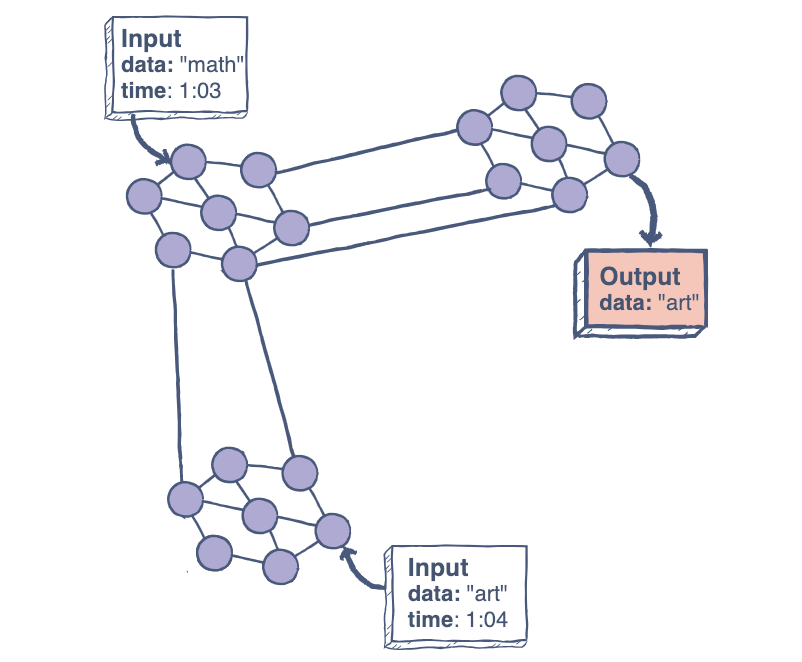
\includegraphics[width=0.8\linewidth]{Photos/HW1/Consistency.png}
        \caption{نمایش سازگاری -
        در اینجا \lr{"art"} آخرین نوشته است.}
        \label{fig:my_label}
    \end{figure}
    اگر یک عملیات خواندن را روی یک سیستم سازگار مانند شکل 1 انجام دهیم، باید آخرین مقدار نوشته شده را برگرداند و این برای همه‌ی نودها برقرار باشد.
    

    \item دسترس‌پذیری
    \lr{(Availability)}\\
    این ویژگی تضمین می‌کند که سیستم همواره عملیاتی باقی بماند؛ یعنی هر درخواست بدون در نظر گرفتن وضعیت مجزای هر نود، پاسخی بدون خطا دریافت می‌کند.
    \begin{figure}[H]
        \centering
        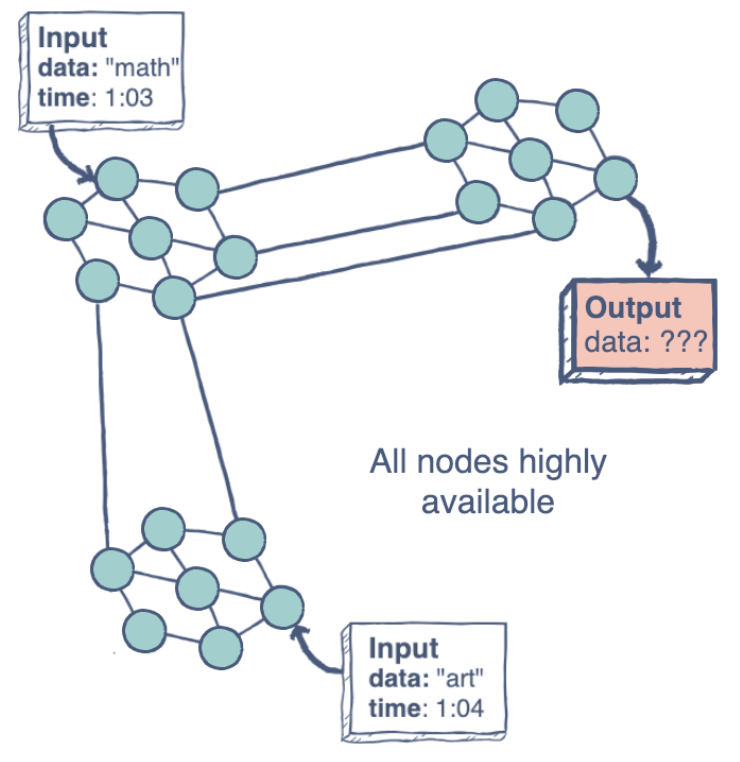
\includegraphics[width=0.65\linewidth]{Photos/HW1/Availability.png}
        \caption{نمایش دسترس‌پذیری -
        پاسخ دریافت نشده و سیستم \lr{unavailable} است.}
        \label{fig:my_label}
    \end{figure}
    این ویژگی، تضمین نمی‌کند که پاسخ حاوی آخرین نوشته باشد.
    
    \item تاب‌آوری
    \lr{(Partition Tolerance)}\\
    بیان می‌کند که صرف‌نظر از اینکه پیام‌ها بین گره‌های یک سیستم حذف شده یا با تأخیر مواجه شوند، سیستم از کار نمی‌افتد. رعایت این مورد در سیستم‌های توزیع‌شده امروزه بسیار ضروری است.
    \begin{figure}[H]
        \centering
        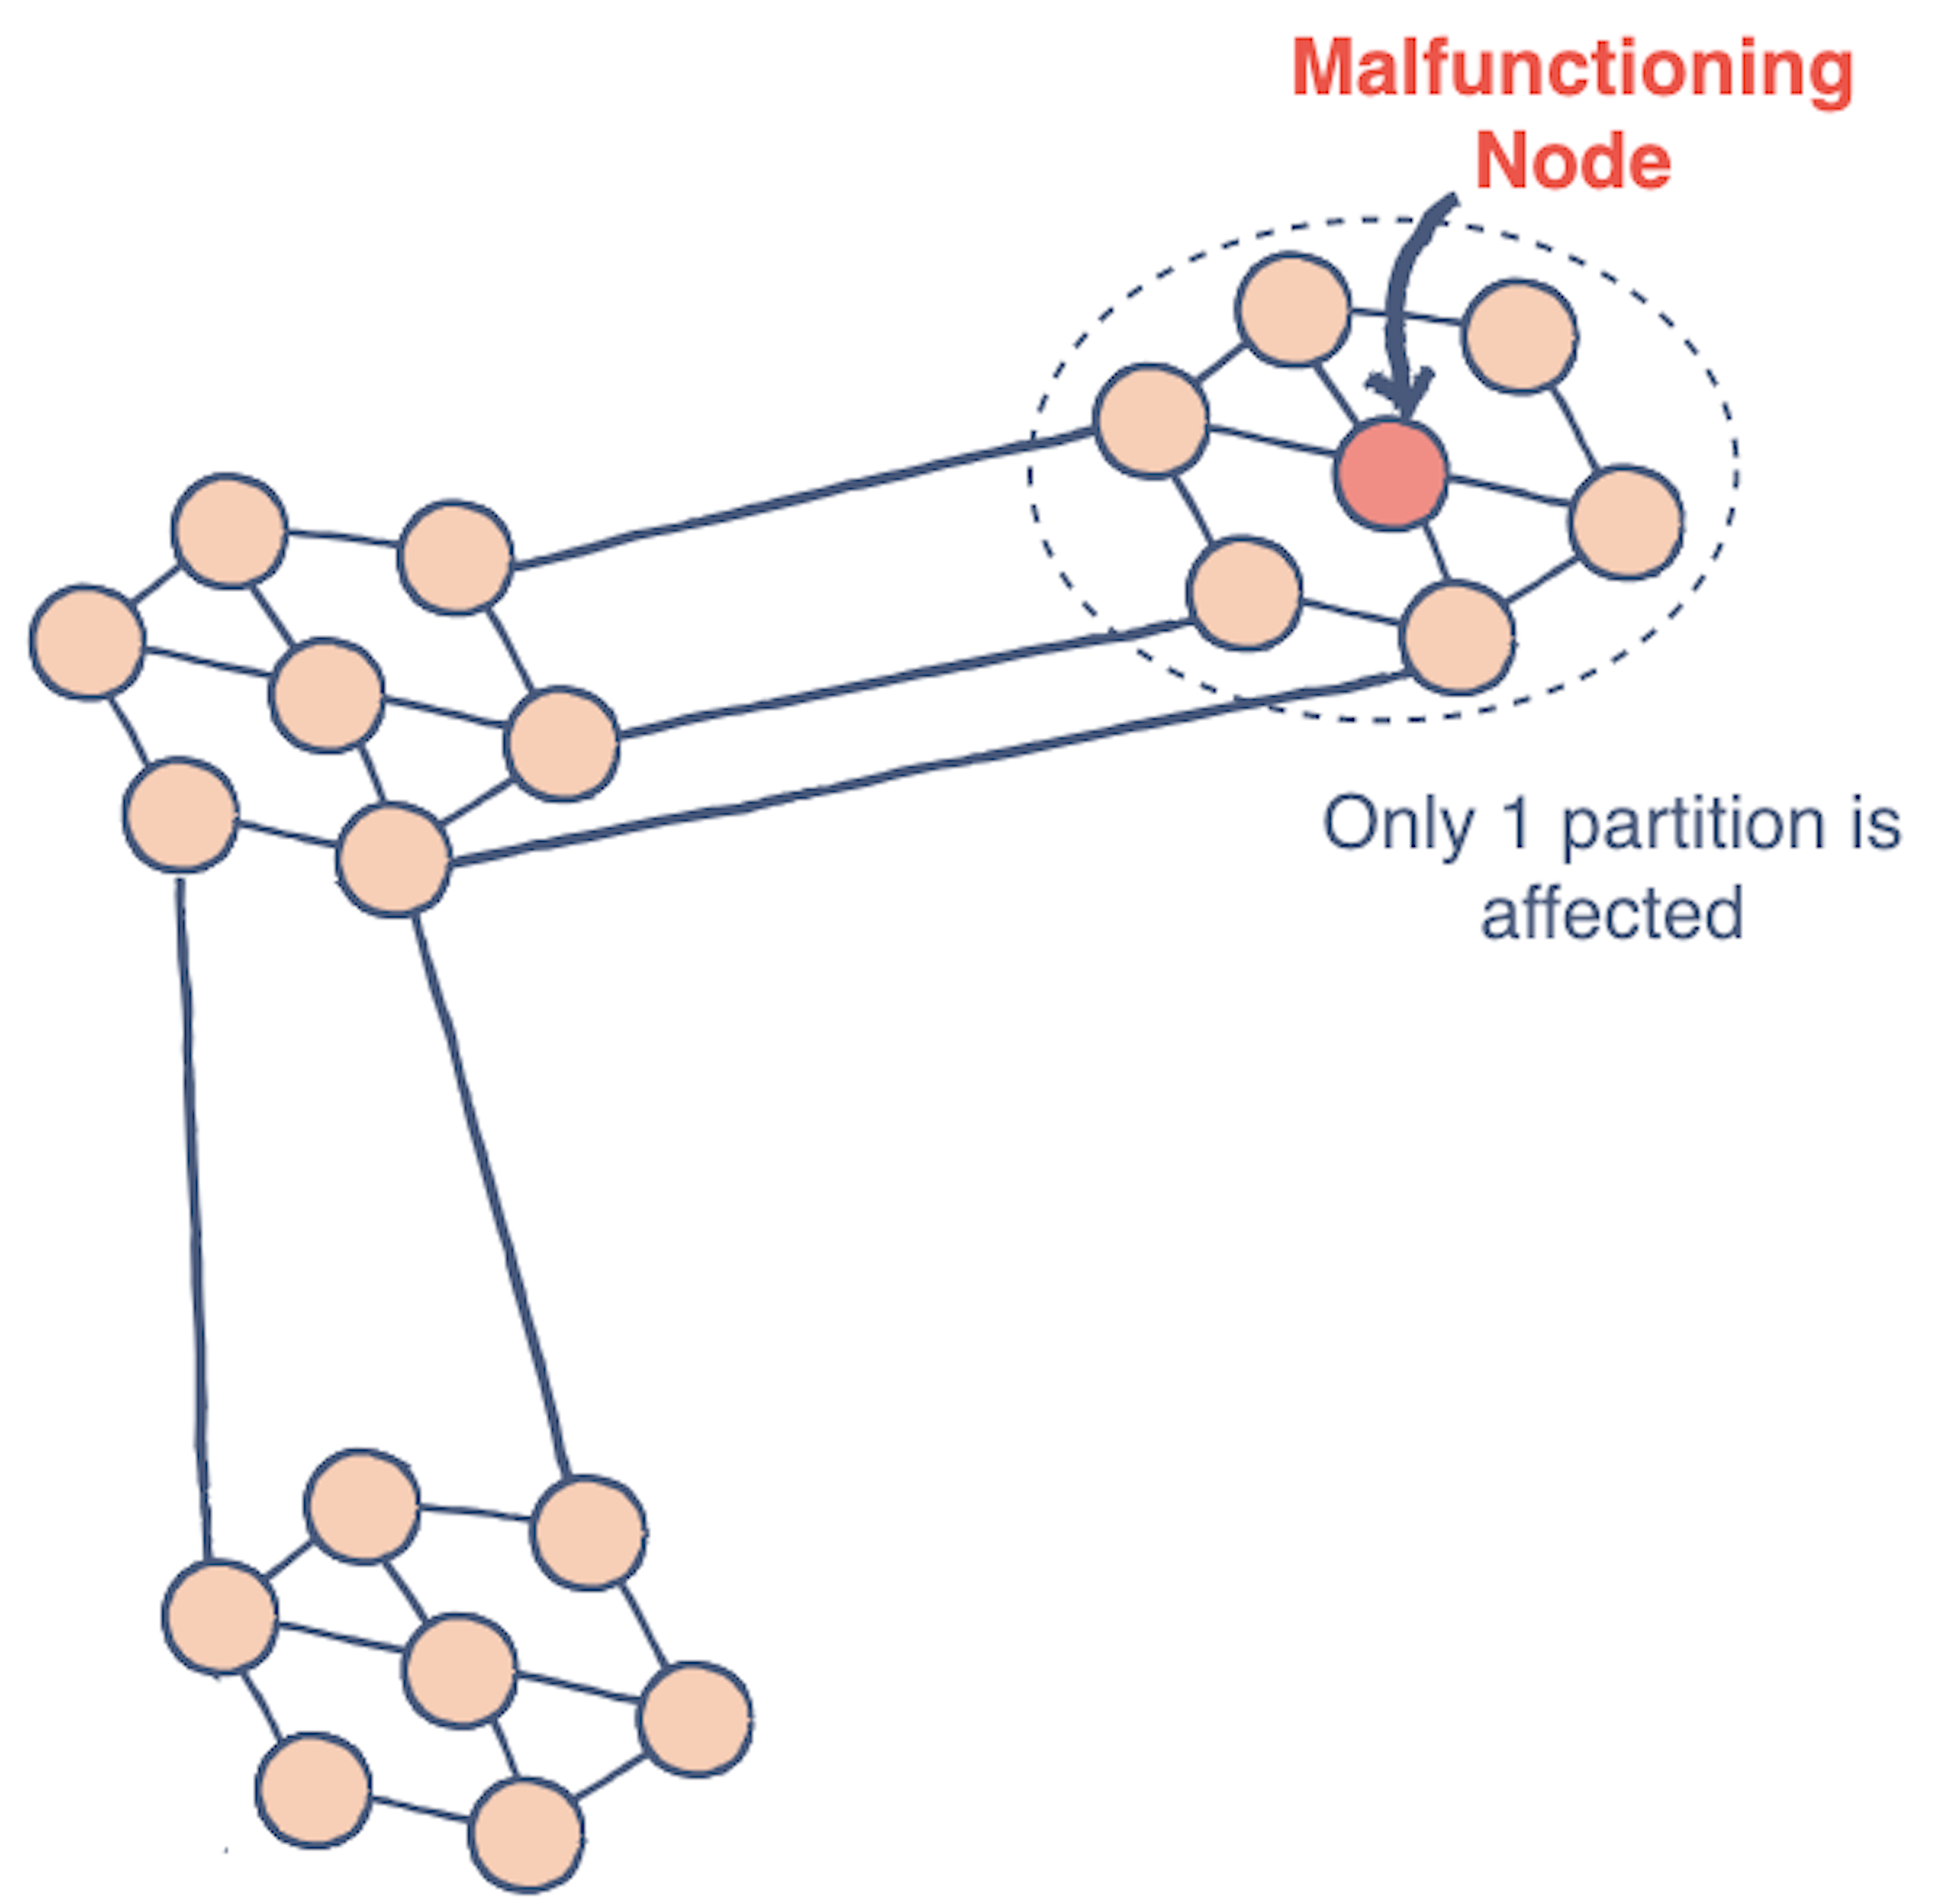
\includegraphics[width=0.6\linewidth]{Photos/HW1/Tolerance.png}
        \caption{نمایش تاب‌آوری -
        عملکرد نادرست یک نود باعث از کار افتادن شبکه نشده است.}
        \label{fig:my_label}
    \end{figure}
    برقراری این ویژگی با تکثیر کافی دیتا در نودهای شبکه امکان‌پذیر است.
    
\end{itemize}

\pagebreak

به طور کل تئوری \lr{CAP} برقراری آخرین (ضروری‌ترین) ویژگی را مدیون فدا شدن یکی از دو ویژگی قبلی می‌داند یا اصطلاحاً باید
\lr{trade-off}
بین \lr{Consistency} و \lr{Availability}
برقرار باشد؛ گرچه امروزه ترجیح ما در طراحی سیستم‌های توزیع‌شده بر پایین آوردن خطای نودها و لینک‌های ارتباطی بین آنها، مثلاً از طریق بک‌آپ گیری یا تقویت سیستم ارتباطات است که در نتیجه‌ی آن تا حد ممکن از این مصالحه بین سازگاری و دسترس‌پذیری اجتناب کنیم.
\rule{\linewidth}{1pt}
\section{رابطه سیستم‌های توزیع‌شده مبتنی بر 
ارسال پیام و مبتنی بر
حافظه مشترک}
همان‌طور که از اسامی برمی‌آید، در مدل \lr{Shared Memory} 
یک منطقه حافظه مشترک وجود دارد که توسط فرآیندها برای ارتباطات استفاده می‌شود و در مدل 
\lr{Message Passing}
فرآیندها از طریق پیوند ارتباطی بین‌شان، عملیات‌های ارسال و دریافت پیام را انجام می‌دهند.
\begin{figure}[H]
        \centering
        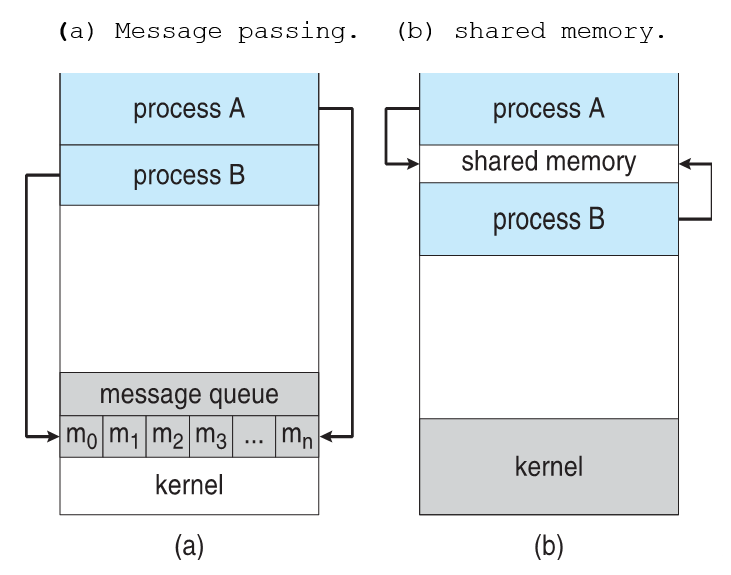
\includegraphics[width=0.8\linewidth]{Photos/HW1/shared-pass.png}
        \caption{ساختار مدل‌های حافظه مشترک و ارسال پیام}
        \label{fig:my_label}
\end{figure}
- برای ساخت یک سیستم ارسال پیام از روی یک سیستم حافظه مشترک، می‌توانیم یک کانال تک‌نویسنده - تک‌خواننده با روش \lr{polling} بسازیم.\\
می‌توان برای هر یال $uv$ در شبکه‌ی ارسال پیام، یک ثبات $r_{uv}$ در نظر گرفت که $u$ هر بار که می‌خواهد عملیات ارسال انجام دهد، دنباله‌ی تمام پیام‌هایی که به $v$ فرستاده را در این ثبات می‌نویسد.\\
از طرفی برای دریافت پیام نیز
$v$
به صورت دوره‌ای به ثبات‌های ورودی سرکشی می‌کند و در صورتی که پیام پردازش نشده‌ای وجود داشته باشد، روند آن را خاتمه می‌دهد.\\
می‌توان اندازه‌ی ثبات مذکور را با استفاده از اضافه کردن یک ثبات کمکی با هدف تأیید دریافت پیام، کاهش داد. بدین صورت که $u$ فقط یک پیام در
$r_{uv}$
بنویسد و باقی پیام‌ها را در صف نگه دارد تا وقتی که $v$ تأیید کند که آن پیام را دریافت کرده است.\\
بدین صورت می‌توان 
$r_{uv}$
را به سه وضعیت ارسال صفر، ارسال یک و  یا شروع مجدد و همچنین ثبات تأیید یا $\text{ack}_{vu}$ را به یک بیت
برای نمایش دریافت مقدار یا شروع مجدد کاهش داد؛ گرچه برای بیشتر کاربردها زیاده‌روی به حساب می‌آید.

- برای ساخت یک سیستم حافظه مشترک از روی یک سیستم ارسال پیام، فرض می‌کنیم سیستم آسنکرون بوده، شبکه کامل است و فقط با
$f<\dfrac{n}{2}$
خرابی سر و کار داریم. همچنین می‌خواهیم ثبات‌های تک‌نویسنده بسازیم.\\
به تعداد $n$ کپی از ثبات درست می‌کنیم. (یکی به ازای هر پردازه) که هرکدام از این کپی‌ها یک زوج‌مرتب
$\left( \text{\lr{value, timestamp}} \right)$
نگه می‌دارد که برای هرکس از صفر شروع می‌شود. \\
یک پروسه کپی خود را در صورت دریافت
$\text{write}\left( v, t \right)$
از پروسه‌ای که $t$ بزرگتری از زمان فعلی وی داشته باشد،
به مقدار جدید
$\left( v, t \right)$
آپدیت می‌کند و با
$\text{ack}\left( v, t \right)$
به پروسه‌ی ارسال کننده، پاسخ می‌دهد که کپی خود را آپدیت کرده است.\\
همچنین در پاسخ به
$\text{read}\left( u \right)$
نیز یک سه‌تایی
$\text{ack}\left( \text{\lr{value, timestamp, u}} \right)$
می‌فرستد که در اینجا $u$
معمولاً ترکیبی از $P_{\text{id}}$ و \text{timestamp} محلی است.\\
برای نوشتن یک مقدار، نویسنده تایم محلی را افزایش می‌دهد و ضمن آپدیت مقدار،
$\text{write}\left(\text{\lr{value, timestamp}} \right)$
را به همه‌ی پردازه‌ها می‌فرستد. عملیات نوشتن، با دریافت تأییدیه از طرف اکثریت پروسه‌ها، به پایان می‌رسد.\\
برای خواندن، خواننده دو قدم دارد:
\begin{enumerate}
  \item ارسال 
  $\text{read}\left( u \right)$
  به همه‌ی پروسه‌ها (که در اینجا $u$ هر مقدار از پیش استفاده نشده‌ای است)
  و انتظار برای دریافت تأییدیه از اکثریت پروسه‌ها.
  \item ارسال
  $\text{write}\left( v, t \right)$
  به همه‌ی پروسه‌ها و انتظار برای دریافت پاسخ
  $\text{ack}\left( v, t \right)$
  از اکثریت پردازه‌ها.
\end{enumerate}
هر دوی خواندن و نوشتن
$\Theta \left( n \right)$
هزینه می‌برند (در واقع
$\Theta \left( 1 \right)$
به ازای هر پروسه).
\begin{figure}[H]
        \centering
        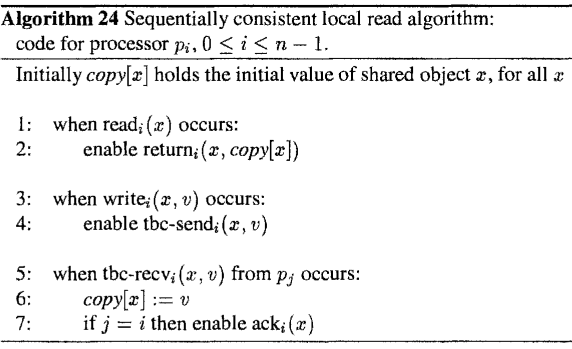
\includegraphics[width=0.75\linewidth]{Photos/HW1/read.PNG}
        \caption{الگوریتم خواندن}
        \label{fig:my_label}
\end{figure}
\begin{figure}[H]
        \centering
        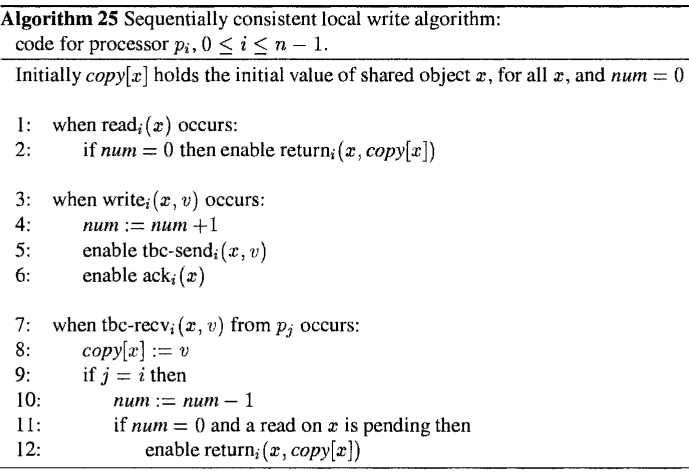
\includegraphics[width=0.8\linewidth]{Photos/HW1/write.PNG}
        \caption{الگوریتم نوشتن}
        \label{fig:my_label}
\end{figure}
\end{multicols}
\end{document}
